\documentclass[a4paper,12pt]{article}
\usepackage[utf8]{inputenc}
\usepackage[german]{babel}
\usepackage{amsmath}
\usepackage{amssymb}
\usepackage{amsthm}
\usepackage{geometry}
\usepackage{graphicx}
\usepackage[hidelinks]{hyperref}
\usepackage{listings}
\usepackage{xcolor}
\usepackage{enumitem}
\usepackage{booktabs}
\usepackage{array}
\usepackage{microtype}

\geometry{margin=2.5cm}

\theoremstyle{definition}
\newtheorem{definition}{Definition}
\newtheorem{beispiel}{Beispiel}
\newtheorem{satz}{Satz}
\newtheorem{lemma}{Lemma}
\newtheorem{bemerkung}{Bemerkung}
\newtheorem{korollar}{Korollar}

\setlist[itemize,1]{label=--}

% ---------- Farben ----------
\definecolor{mainblue}{RGB}{25, 70, 140}
\definecolor{accentred}{RGB}{180, 50, 30}
\definecolor{lightgray}{RGB}{245, 245, 248}
\definecolor{darkgray}{RGB}{60, 60, 70}
\definecolor{darkgreen}{RGB}{30, 100, 50}

\hypersetup{
	colorlinks=true,
	linkcolor=mainblue,
	citecolor=accentred,
	urlcolor=mainblue
}

\lstset{
	basicstyle=\ttfamily\small,
	keywordstyle=\color{blue},
	commentstyle=\color{gray},
	stringstyle=\color{accentred},
	numbers=left,
	numberstyle=\tiny,
	breaklines=true,
	frame=single,
	literate=%
	{Ö}{{\"O}}1
	{Ä}{{\"A}}1
	{Ü}{{\"U}}1
	{ß}{{\ss}}1
	{ü}{{\"u}}1
	{ä}{{\"a}}1
	{ö}{{\"o}}1
}

\title{\textbf{FLEX-Standard:}\\[0.4em]
Ein formaler Standard für lose Kopplung von\\
Suchdiensten und Web-Service-Ketten\\
in mobilen Applikationen\\[0.6em]
{\large mit qualitätserhaltendem Wettbewerbsmodell\\[0.2em]
und Schnittstellenkompatibilität via Subgraph Algorithmus}}
\author{Stephan Epp\\[0.3em]
{}
\date{Mai 2026}

\begin{document}

\maketitle

\begin{abstract}
\noindent
Mobile Applikationen greifen heute auf eine Vielzahl externer Dienste zurück: Suchmaschinen, Spracherkennung (Speech-to-Text, STT), Sprachsynthese (Text-to-Speech, TTS), Übersetzungsdienste und Natural Language Processing (NLP). Die feste Verdrahtung dieser Dienste führt zu Anbieterabhängigkeit, mangelnder Anpassungsfähigkeit an regionale Regulatorik und zu suboptimaler Dienstqualität. Diese Arbeit stellt den \textbf{FLEX-Standard} (Flexible Loose-coupled EXchangeable Services) vor: ein formales Framework für die lose Kopplung und den dynamischen Austausch von Suchdiensten und Web-Service-Ketten in mobilen Applikationen. FLEX definiert eine graphbasierte Schnittstellenspezifikation, deren Kompatibilität mit dem Subgraph Algorithmus (Epp 2026) in $O(n^3)$ entschieden wird. Ein mehrdimensionales QoS-Modell bildet die Grundlage für ein vierteljährliches Wettbewerbsmodell, das Qualitätssicherung und Wettbewerbserhalt systematisch gewährleistet. Für die zentrale Routingfunktion werden formale Korrektheit, Eindeutigkeit und Komplexitätsoptimalität bewiesen. Matplotlib-Visualisierungen illustrieren QoS-Zeitverläufe, regionale Routing-Entscheidungen, Kettenlatenz und Wettbewerbsevolution.
\end{abstract}

\tableofcontents
\newpage

% =============================================================
\section{Einführung}
% =============================================================

\subsection{Problemstellung}

Moderne mobile Applikationen sind auf externe Dienste angewiesen, die sie bisher typischerweise fest in den Quellcode einbetten. Eine Navigations-App nutzt Google Maps als feste Suche; ein Sprachassistent delegiert STT-Aufgaben ausschließlich an Google Cloud Speech oder AWS Transcribe; ein Übersetzungstool ist hart mit DeepL oder Google Translate verdrahtet. Diese enge Kopplung erzeugt ein Bündel fundamentaler Probleme:

\begin{enumerate}
    \item \textbf{Anbieterabhängigkeit (Vendor Lock-in):} Wechsel zu einem alternativen Anbieter erfordert tief greifende Code-Änderungen.
    \item \textbf{Regulatorische Starrheit:} In bestimmten Regionen und Ländern sind einzelne Suchanbieter gesperrt oder unterliegen Datenschutzauflagen (z.\,B.\ DSGVO in der EU, Netzsouveränität in der VR China). Fest integrierte Dienste können diese Auflagen nicht dynamisch erfüllen.
    \item \textbf{Bandbreitenblindheit:} In Niedrigbandbreitenregionen sind latenzarme, leichtgewichtige Dienstalternativen vorzuziehen; fest verdrahtete Dienste ignorieren diesen Kontext.
    \item \textbf{Qualitätsstagnation:} Ohne Wettbewerb haben Anbieter wenig Anreiz zur Qualitätsverbesserung; fest integrierte Dienste profitieren von Trägheitseffekten.
    \item \textbf{Nicht-Kompatibilität in Service-Ketten:} Wenn ein TTS-Dienst durch einen anderen ersetzt werden soll, fehlt eine formale Schnittstellendefinition, die Austauschbarkeit ohne Anpassungsaufwand garantiert.
\end{enumerate}

Diese fünf Probleme sind nicht isoliert. Sie greifen ineinander und erzeugen ein \emph{strukturelles Defizit} in der Architektur moderner mobiler Applikationen: die Abwesenheit eines offenen, formalen Standards für die lose Kopplung externer Dienste.

\subsection{Motivation und Zielsetzung}

Der \textbf{FLEX-Standard} (Flexible Loose-coupled EXchangeable Services) adressiert dieses strukturelle Defizit durch drei koordinierte Mechanismen:

\begin{enumerate}
    \item \textbf{Graphbasierte Schnittstellenspezifikation:} Jede Dienstklasse (Suchmaschine, TTS, STT, Translate, NLP) wird als gerichteter Graph $G_I = (V_I, E_I)$ modelliert, wobei Knoten Datentypen und Kanten Transformationen repräsentieren. Die Kompatibilitätsprüfung zwischen einem Dienst und einer Schnittstelle wird als Subgraph-Problem formuliert und durch den Subgraph Algorithmus (Epp 2026) in $O(n^3)$ entschieden.
    \item \textbf{Dynamisches Routing:} Eine formale Routing-Funktion $R: \mathcal{T}_C \times \mathcal{G} \times \mathcal{B} \to 2^{\mathcal{S}}$ wählt aus dem Raum kompatibler Dienste denjenigen mit optimalem gewichtetem QoS-Score aus, abhängig von Inhaltstyp, geografischer Region und Bandbreitenklasse.
    \item \textbf{Quartalsweises Wettbewerbsmodell:} Alle 90 Tage werden alle registrierten Dienstanbieter anhand eines mehrdimensionalen QoS-Vektors bewertet und nach Score gerankt. Die mobile App nutzt automatisch den bestplatzierten Anbieter, ohne dass der Nutzer dies explizit steuert.
\end{enumerate}

\subsection{Beiträge dieser Arbeit}

Diese Arbeit leistet die folgenden formalen und angewandten Beiträge:

\begin{enumerate}
    \item Vollständige formale Definition des FLEX-Standards mit zehn Kerndefinitionen (Abschnitt~\ref{sec:grundlagen}).
    \item Beweis, dass Schnittstellenkompatibilität in $O(n^3)$ entscheidbar ist (Lemma~\ref{lem:kompatibilitaet}).
    \item Beweis der Wohldefiniertheit und Eindeutigkeit der FLEX-Routing-Funktion (Satz~\ref{satz:eindeutigkeit}).
    \item Beweis der Optimalität der Greedy-Kettenkomposition unter Unabhängigkeitsannahme (Satz~\ref{satz:optimalitaet_kette}).
    \item Beweis der Konvergenz des Wettbewerbsmodells zu einer Pareto-optimalen Anbietermenge (Satz~\ref{satz:konvergenz}).
    \item FLEX-Qualitätsgarantie für zusammengesetzte Dienstketten (Satz~\ref{satz:qualitaet}).
    \item Fünf Matplotlib-Visualisierungen zur empirischen Illustration der formalen Ergebnisse.
\end{enumerate}

% =============================================================
\section{Grundlagen und Definitionen}
\label{sec:grundlagen}
% =============================================================

\subsection{Dienste und Schnittstellen}

\begin{definition}[Dienst]
\label{def:dienst}
Ein \emph{Dienst} ist ein Tupel
\[
    S = (\mathcal{I}_S,\; \mathcal{O}_S,\; \mathcal{P}_S,\; \mathcal{C}_S,\; G_S)
\]
wobei
\begin{itemize}
    \item $\mathcal{I}_S$ die Menge der akzeptierten Eingabetypen ist,
    \item $\mathcal{O}_S$ die Menge der produzierten Ausgabetypen ist,
    \item $\mathcal{P}_S \subset \mathbb{R}^k$ der QoS-Parameterraum mit $k$ Dimensionen ist,
    \item $\mathcal{C}_S \subseteq \mathcal{G} \times \mathcal{B}$ die Menge zulässiger \mbox{(Region, Bandbreite)}-Paare ist, und
    \item $G_S = (V_S, E_S)$ der gerichtete Fähigkeitsgraph des Dienstes ist.
\end{itemize}
\end{definition}

\begin{definition}[Schnittstelle]
\label{def:schnittstelle}
Eine \emph{Schnittstelle} ist ein Tupel
\[
    I = (G_I,\; T_I,\; \tau_I)
\]
wobei
\begin{itemize}
    \item $G_I = (V_I, E_I)$ der gerichtete Operationsgraph der Schnittstelle ist,
    \item $T_I: V_I \to \mathcal{T}$ eine Typisierungsfunktion ist, die jedem Knoten einen Datentyp zuweist, und
    \item $\tau_I \subseteq V_I$ die Menge der Terminalknoten (Ausgabeknoten) ist.
\end{itemize}
\end{definition}

Im Operationsgraphen $G_I$ repräsentiert jeder Knoten $v \in V_I$ einen Datentyp (z.\,B.\ Audiodaten, UTF-8-Text, JSON-Objekt), und jede gerichtete Kante $(u, v) \in E_I$ repräsentiert eine Transformation, die den Typ $T_I(u)$ in den Typ $T_I(v)$ überführt.

\begin{beispiel}[STT-Schnittstelle]
Die STT-Schnittstelle $I_{\mathrm{STT}}$ hat den Operationsgraphen:
\[
G_{I_{\mathrm{STT}}} = \bigl(\{\text{Audio}, \text{Text}\},\; \{(\text{Audio}, \text{Text})\}\bigr)
\]
mit $T_{I_{\mathrm{STT}}}(\text{Audio}) = \texttt{PCM}$, $T_{I_{\mathrm{STT}}}(\text{Text}) = \texttt{UTF-8}$ und $\tau_{I_{\mathrm{STT}}} = \{\text{Text}\}$.
\end{beispiel}

\begin{definition}[Schnittstellenkompatibilität]
\label{def:kompatibilitaet}
Ein Dienst $S$ \emph{implementiert} eine Schnittstelle $I$, geschrieben $S \models I$, wenn der Operationsgraph der Schnittstelle ein Subgraph des Fähigkeitsgraphen des Dienstes ist:
\[
    S \models I \;\iff\; G_I \subseteq G_S
\]
d.\,h.\ $V_I \subseteq V_S$ und $E_I \subseteq E_S$ (nach geeigneter Knotenidentifikation via Typisierung).
\end{definition}

\subsection{QoS-Modell}

\begin{definition}[QoS-Vektor]
\label{def:qos}
Der \emph{QoS-Vektor} eines Dienstes $S$ ist eine Abbildung
\[
    \mathbf{q}: \mathcal{S} \times \mathcal{T} \to [0,1]^k, \quad \mathbf{q}(S, t) = (q_1(S,t), \ldots, q_k(S,t))
\]
wobei $\mathcal{T}$ die Menge der Messzeitpunkte ist und die $k$ Komponenten folgende Qualitätsdimensionen messen:
\begin{align*}
q_1 &: \text{normalisierte inverse Latenz} \quad (1 - L/L_{\max}), \\
q_2 &: \text{Erkennungsgenauigkeit} \quad (F_1\text{-Score}), \\
q_3 &: \text{Verfügbarkeit} \quad (\text{Uptime-Prozentsatz} / 100), \\
q_4 &: \text{Datenschutzkonformität} \quad (\in \{0, 0.5, 1\}), \\
q_5 &: \text{Kosteneffizienz} \quad (1 - \mathrm{Kosten}/\mathrm{Kosten}_{\max}).
\end{align*}
\end{definition}

\begin{definition}[Gewichteter QoS-Score]
\label{def:score}
Gegeben ein Gewichtsvektor $\mathbf{w} = (w_1, \ldots, w_k)$ mit $\sum_{i=1}^k w_i = 1$, $w_i \geq 0$, ist der \emph{gewichtete QoS-Score} eines Dienstes $S$ zum Zeitpunkt $t$:
\[
    Q_{\mathbf{w}}(S, t) \;=\; \sum_{i=1}^{k} w_i \cdot q_i(S, t) \;\in\; [0, 1].
\]
\end{definition}

\begin{definition}[Geografische Region]
\label{def:region}
Eine \emph{geografische Region} $g \in \mathcal{G}$ ist ein Element einer endlichen Partition der Erdoberfläche, die durch Länder, Rechtsjurisdiktionen und Netzwerktopologien bestimmt wird. Für jede Region $g$ existiert eine Menge $\mathcal{L}(g) \subseteq \mathcal{S}$ zulässiger Dienste (regulatorische Whitelist).
\end{definition}

\begin{definition}[Bandbreitenklasse]
\label{def:bandbreite}
Die \emph{Bandbreitenklasse} $b \in \mathcal{B} = \{B_\mathrm{low}, B_\mathrm{med}, B_\mathrm{high}\}$ klassifiziert die verfügbare Netzwerkbandbreite:
\[
    B_\mathrm{low} = [0, 10)\;\mathrm{Mbit/s}, \quad
    B_\mathrm{med} = [10, 50)\;\mathrm{Mbit/s}, \quad
    B_\mathrm{high} = [50, \infty)\;\mathrm{Mbit/s}.
\]
Jedem Dienst $S$ ist ein Minimalanforderungsvektor $\mathbf{b}_{\min}(S) \in \mathcal{B}$ zugeordnet.
\end{definition}

\subsection{Routing und Dienstketten}

\begin{definition}[Routing-Funktion]
\label{def:routing}
Die \emph{FLEX-Routing-Funktion} ist eine Abbildung
\[
    R: \mathcal{T}_C \times \mathcal{G} \times \mathcal{B} \to \mathcal{S}
\]
wobei $\mathcal{T}_C$ die Menge der Inhaltstypen (z.\,B.\ Websuche, Sprachanfrage, Dokumentübersetzung) ist. Sie wählt für einen gegebenen Kontext $(c, g, b)$ den Dienst mit maximalem gewichtetem QoS-Score aus der Menge der kompatiblen und regulatorisch zulässigen Dienste:
\[
    R(c, g, b) = \argmax_{S \in \mathcal{C}(c,g,b)} Q_{\mathbf{w}(c)}(S, t_{\mathrm{akt}})
\]
wobei $\mathcal{C}(c,g,b) = \{S \in \mathcal{S} \mid S \models I(c),\; g \in \mathcal{G}(S),\; b \succeq \mathbf{b}_{\min}(S)\}$ die Kandidatenmenge ist.
\end{definition}

\begin{definition}[Dienstkette]
\label{def:kette}
Eine \emph{Dienstkette} der Länge $m$ ist eine Sequenz
\[
    \mathcal{K} = (S_1, S_2, \ldots, S_m)
\]
von Diensten. Sie ist \emph{gültig} (kettenkompatibel) wenn für alle $i \in \{1, \ldots, m-1\}$ gilt:
\[
    \mathcal{O}_{S_i} \cap \mathcal{I}_{S_{i+1}} \neq \emptyset.
\]
\end{definition}

\begin{beispiel}[STT-Translate-TTS-Kette]
Die Kette $\mathcal{K} = (\mathrm{STT}, \mathrm{Trans}, \mathrm{TTS})$ ist gültig, da:
\begin{itemize}
    \item $\mathcal{O}_\mathrm{STT} = \{\texttt{UTF-8}\} \cap \mathcal{I}_\mathrm{Trans} = \{\texttt{UTF-8}\} \neq \emptyset$,
    \item $\mathcal{O}_\mathrm{Trans} = \{\texttt{UTF-8}\} \cap \mathcal{I}_\mathrm{TTS} = \{\texttt{UTF-8}\} \neq \emptyset$.
\end{itemize}
\end{beispiel}

\begin{definition}[Wettbewerbsintervall und Wettbewerbsscore]
\label{def:wettbewerb}
Das \emph{Wettbewerbsintervall} hat die Dauer $\Delta T = 90$ Tage. Der \emph{Wettbewerbsscore} eines Dienstanbieters $S$ für das $r$-te Wettbewerbsintervall $[t_{r-1}, t_r]$ ist der zeitliche Mittelwert des gewichteten QoS-Scores:
\[
    Q_{\mathrm{comp}}(S, r) = \frac{1}{t_r - t_{r-1}} \int_{t_{r-1}}^{t_r} Q_{\mathbf{w}}(S, t)\, dt
    \;\approx\; \frac{1}{|\mathcal{M}_r|} \sum_{t \in \mathcal{M}_r} Q_{\mathbf{w}}(S, t)
\]
wobei $\mathcal{M}_r$ die Menge der Messpunkte im Intervall $r$ ist.
\end{definition}

% =============================================================
\section{Das FLEX-Standard-Framework}
\label{sec:flex}
% =============================================================

\subsection{Architekturübersicht}

Der FLEX-Standard definiert eine dreischichtige Architektur zwischen mobiler Applikation und konkreten Dienstanbietern:

\begin{center}
\begin{tabular}{|c|}
\hline
\rule{0pt}{2.2ex}\textbf{Mobile Applikation (Nutzerebene)}\\
\hline
\rule{0pt}{2.2ex}FLEX-Abstraktionsschicht (Routing, Kompatibilität, QoS)\\
\hline
\rule{0pt}{2.2ex}Konkrete Dienstanbieter (Google, Bing, AWS, DeepL, \ldots)\\
\hline
\end{tabular}
\end{center}

\medskip
\noindent
Die \emph{mobile Applikation} kommuniziert ausschließlich mit der FLEX-Abstraktionsschicht über normierte Schnittstellen $I \in \{I_\mathrm{Search}, I_\mathrm{TTS}, I_\mathrm{STT}, I_\mathrm{Trans}, I_\mathrm{NLP}\}$. Für den Nutzer ist der konkrete Anbieter transparent.

\subsection{Schnittstellenspezifikation}

Die fünf FLEX-Standardschnittstellen sind in Tabelle~\ref{tab:interfaces} zusammengefasst.

\begin{table}[h]
\centering
\caption{FLEX-Standardschnittstellen}
\label{tab:interfaces}
\begin{tabular}{llll}
\toprule
Schnittstelle & Eingabetyp & Ausgabetyp & Beispielanbieter \\
\midrule
$I_\mathrm{Search}$ & \texttt{UTF-8-Query} & \texttt{JSON-Results} & Google, Bing, DDG \\
$I_\mathrm{TTS}$    & \texttt{UTF-8-Text} & \texttt{PCM-Audio} & Azure Cognitive, Google TTS \\
$I_\mathrm{STT}$    & \texttt{PCM-Audio} & \texttt{UTF-8-Text} & AWS Transcribe, Whisper \\
$I_\mathrm{Trans}$  & \texttt{UTF-8-Text} & \texttt{UTF-8-Text} & DeepL, LibreTranslate \\
$I_\mathrm{NLP}$    & \texttt{UTF-8-Text} & \texttt{JSON-NLP} & Google NLP, Azure NLP \\
\bottomrule
\end{tabular}
\end{table}

\subsection{Inhaltsbasiertes Routing}

Der FLEX-Standard klassifiziert eingehende Anfragen automatisch nach Inhaltstyp $c \in \mathcal{T}_C$. Ein Klassifikator $\kappa: \mathcal{X} \to \mathcal{T}_C$ ordnet jeder Rohanfrage $x \in \mathcal{X}$ den Inhaltstyp zu. Auf Basis dieses Typs wird die zugehörige Schnittstelle $I(c)$ aktiviert und der Routing-Algorithmus gestartet.

Das kontextabhängige Gewicht $\mathbf{w}(c)$ im QoS-Score (Definition~\ref{def:score}) ist für jeden Inhaltstyp anders kalibriert: Bei Echtzeit-STT dominiert $w_1$ (Latenz), bei Dokumentenübersetzung dominiert $w_2$ (Genauigkeit) und $w_4$ (Datenschutz).

\subsection{Geographisches Routing}

Für jede geografische Region $g$ und jeden Inhaltstyp $c$ pflegt der FLEX-Standard eine vorkompilierte \emph{Zulässigkeitsmenge} $\mathcal{L}(g, c)$ zulässiger Dienste. Diese Menge wird durch:

\begin{itemize}
    \item Regulatorische Datenbanken (DSGVO-Konformität, nationale Sperrlisten),
    \item Netzwerkreichabilitätsmessungen (latenzbasiert, DNS-Auflösung),
    \item Datenschutzzertifizierungen (ISO 27001, SOC 2)
\end{itemize}

quartalsweise aktualisiert. Bei jeder Routing-Anfrage wird $\mathcal{C}(c,g,b) \subseteq \mathcal{L}(g,c)$ berechnet.

\subsection{Dienstkettenkomposition}

Für mehrstufige Anfragen (z.\,B.\ Sprachanfrage in Fremdsprache mit Sprachausgabe) komponiert der FLEX-Standard automatisch eine gültige Dienstkette. Der Kompositionsalgorithmus~\ref{alg:kette} wählt für jede Stufe $i$ den Dienst mit maximalem QoS-Score aus.

\begin{lstlisting}[caption={FLEX-CHAIN-COMPOSE: Greedy-Kettenkomposition},label={alg:kette},language=Python]
def flex_chain_compose(requirements, g, b, w):
    """
    requirements: Liste von Schnittstellentypen [I_1, .., I_m]
    g: geografische Region
    b: Bandbreitenklasse
    w: Gewichtsvektor
    """
    chain = []
    for interface in requirements:
        # Kandidatenmenge: kompatibel, zulaessig, bandbreitentauglich
        candidates = [S for S in REGISTRY
                      if S.implements(interface)
                      and g in S.regions
                      and b >= S.min_bandwidth]
        if not candidates:
            raise NoServiceAvailableError(interface)
        # Wähle Dienst mit maximalem QoS-Score
        best = max(candidates, key=lambda S: qos_score(S, w))
        chain.append(best)
    return chain
\end{lstlisting}

\subsection{Wettbewerbsmodell}

Am Ende jedes Wettbewerbsintervalls $\Delta T = 90$ Tage führt der FLEX-Standard eine Wettbewerbsevaluation durch:

\begin{lstlisting}[caption={FLEX-COMPETITION-RANK: Wettbewerbsrankierung},label={alg:wettbewerb},language=Python]
def flex_competition_rank(providers, r, w, q_min=0.80):
    """
    providers: Menge aller registrierten Anbieter
    r: aktuelles Wettbewerbsintervall
    q_min: Mindestscore-Schwelle
    """
    scores = {S: competition_score(S, r) for S in providers}
    # Disqualifikation unter Mindestschwelle
    qualified = {S: sc for S, sc in scores.items() if sc >= q_min}
    # Ranking nach Score
    ranking = sorted(qualified, key=qualified.get, reverse=True)
    # Update des FLEX-Registry mit neuem Routing-Ranking
    update_registry_ranking(ranking)
    return ranking
\end{lstlisting}

Anbieter, deren $Q_\mathrm{comp}(S, r) < q_{\min}$ fällt, werden aus der Kandidatenmenge $\mathcal{C}$ für das nächste Quartal ausgeschlossen, bis sie die Schwelle wieder überschreiten.

% =============================================================
\section{Schnittstellenkompatibilität via Subgraph Algorithmus}
\label{sec:subgraph}
% =============================================================

\subsection{Graphmodellierung der Kompatibilität}

Die zentrale Prüfung im FLEX-Standard ist, ob ein Dienst $S$ eine Schnittstelle $I$ implementiert, d.\,h.\ ob $G_I \subseteq G_S$ gilt (Definition~\ref{def:kompatibilitaet}). Diese Frage ist ein Sonderfall des allgemeinen Subgraph-Isomorphie-Problems, das NP-vollständig ist. Für die strukturierte Klasse der FLEX-Schnittstellen (DAGs mit typisierter Knotenidentifikation) ist das Problem jedoch in polynomieller Zeit lösbar.

Der Subgraph Algorithmus (Epp 2026) \cite{epp2026} entscheidet dieses Problem für Graphen mit $n$ Knoten in $O(n^3)$ durch:

\begin{enumerate}
    \item Berechnung eindeutiger Signaturen $\sigma_j = \sum_{i=0}^{n-1} A_{ij} \cdot 2^i + j \cdot 2^n$ für jede Spalte $j$ der Adjazenzmatrix,
    \item Zyklische Rotation der Signatursequenz (nur $n$ Rotationen statt $n!$ Permutationen),
    \item LCS-Vergleich der Signatursequenzen für jede Rotation.
\end{enumerate}

\subsection{Formale Kompatibilitätsprüfung}

\begin{lemma}[Schnittstellenkompatibilität in $O(n^3)$]
\label{lem:kompatibilitaet}
Sei $I = (G_I, T_I, \tau_I)$ eine FLEX-Schnittstelle mit $n_I = |V_I|$ Knoten und $S$ ein Dienst mit Fähigkeitsgraph $G_S$ mit $n_S = |V_S|$ Knoten, $n_I \leq n_S$. Die Frage $S \models I$ (d.\,h.\ $G_I \subseteq G_S$) ist in Zeit $O(n_S^3)$ entscheidbar.
\end{lemma}

\begin{proof}
Wir reduzieren die Kompatibilitätsprüfung auf das Subgraph-Problem und wenden den Subgraph Algorithmus (Epp 2026, Satz~2) an.

\textbf{Schritt 1: Knotenidentifikation via Typisierung.} Da FLEX-Schnittstellen typisiert sind, können Knoten von $G_I$ und $G_S$ über ihre Typen $T_I, T_S$ identifiziert werden. Definiere die Knotenabbildung $\varphi: V_I \to V_S$ mit $\varphi(v) = u$ falls $T_I(v) = T_S(u)$. Diese Abbildung ist eindeutig, da die Typen paarweise verschieden sind (Eindeutigkeitsannahme des FLEX-Standards).

\textbf{Schritt 2: Reduktion auf Adjazenzmatrizen.} Repräsentiere $G_I$ durch Adjazenzmatrix $A \in \{0,1\}^{n_I \times n_I}$ und $G_S$ durch $B \in \{0,1\}^{n_S \times n_S}$. Die Knotenidentifikation via $\varphi$ induziert eine Einbettung von $A$ in $B$.

\textbf{Schritt 3: Anwendung des Subgraph Algorithmus.} Nach Epp (2026) entscheidet der Subgraph Algorithmus durch Berechnung von Signaturvektoren und LCS-Vergleich über $n_S$ zyklische Rotationen, ob $G_I \subseteq G_S$. Die Gesamtkomplexität beträgt $O(n_S^3)$ (Signaturberechnung: $O(n_S^2)$; LCS pro Rotation: $O(n_S^2)$; $n_S$ Rotationen: Gesamt $O(n_S^3)$).

\textbf{Korrektheit:} Die Injektivität der Signaturfunktion (Lemma~1 in Epp 2026) garantiert, dass gleiche Spaltenvektoren identisch signiert werden. Damit liefert der LCS-Vergleich genau dann eine Übereinstimmung, wenn $G_I$ als Subgraph in $G_S$ enthalten ist. $
$
\end{proof}

\begin{lemma}[Kettenvalidierung in $O(m \cdot n^3)$]
\label{lem:kettenvalidierung}
Sei $\mathcal{K} = (S_1, \ldots, S_m)$ eine Dienstkette. Die Validierung aller $m-1$ Kompatibilitätsbedingungen $\mathcal{O}_{S_i} \cap \mathcal{I}_{S_{i+1}} \neq \emptyset$ ist in Zeit $O(m \cdot n^3)$ durchführbar, wobei $n = \max_i |V_{S_i}|$.
\end{lemma}

\begin{proof}
Jede der $m-1$ Kompatibilitätsprüfungen entspricht einer Subgraph-Frage für die Ausgabe-Schnittstelle von $S_i$ in der Eingabe-Schnittstelle von $S_{i+1}$. Nach Lemma~\ref{lem:kompatibilitaet} kostet jede Prüfung $O(n^3)$. Gesamt: $(m-1) \cdot O(n^3) = O(m \cdot n^3)$. $
$
\end{proof}

\begin{bemerkung}
In der Praxis sind die Schnittstellen-Graphen sehr klein ($n_I \leq 10$), sodass die Kompatibilitätsprüfung in konstanter Zeit abläuft und den Routing-Overhead nicht dominiert. Die asymptotische Analyse bleibt dennoch von theoretischer Bedeutung für die Skalierbarkeit bei komplexen, zusammengesetzten Diensten.
\end{bemerkung}

% =============================================================
\section{Formale Analyse des FLEX-Standards}
\label{sec:analyse}
% =============================================================

\subsection{Wohldefiniertheit und Eindeutigkeit der Routing-Funktion}

\begin{satz}[Wohldefiniertheit und Eindeutigkeit]
\label{satz:eindeutigkeit}
Die FLEX-Routing-Funktion $R: \mathcal{T}_C \times \mathcal{G} \times \mathcal{B} \to \mathcal{S}$ ist wohldefiniert und eindeutig für jeden Kontext $(c, g, b)$.
\end{satz}

\begin{proof}
\textbf{Existenz (Wohldefiniertheit):} Für jeden Kontext $(c, g, b)$ enthält die Kandidatenmenge $\mathcal{C}(c, g, b)$ mindestens den \emph{FLEX-Fallback-Dienst} $S_\mathrm{fb}^{(c)}$, der für alle Regionen, alle Bandbreitenklassen und jede FLEX-Standardschnittstelle kompatibel ist. Damit gilt $|\mathcal{C}(c,g,b)| \geq 1$ für alle $(c,g,b) \in \mathcal{T}_C \times \mathcal{G} \times \mathcal{B}$.

\textbf{Eindeutigkeit:} Angenommen, zwei Dienste $S, S' \in \mathcal{C}(c,g,b)$ erfüllen $Q_{\mathbf{w}(c)}(S) = Q_{\mathbf{w}(c)}(S')$. In diesem Fall bricht der FLEX-Standard die Unentschieden-Situation durch lexikografischen Vergleich des Registrierungs-Timestamps auf: Der früher registrierte Anbieter wird bevorzugt. Dies ist eine deterministische totale Ordnung auf $\mathcal{S}$. Damit ist $\argmax$ eindeutig. $
$
\end{proof}

\subsection{Komplexität der Dienstauswahl}

\begin{satz}[Komplexität der Dienstauswahl]
\label{satz:komplexitaet_routing}
Gegeben $|\mathcal{C}(c,g,b)| = N$ Kandidaten und $k$ QoS-Dimensionen, läuft die Berechnung von $R(c,g,b)$ in Zeit $O(N \cdot k + N \log N)$.
\end{satz}

\begin{proof}
Die Berechnung von $Q_{\mathbf{w}(c)}(S, t)$ für einen Dienst erfordert $k$ Multiplikationen und $k-1$ Additionen: $O(k)$. Für alle $N$ Kandidaten: $O(N \cdot k)$. Die Bestimmung des Maximums benötigt $O(N)$ (linearer Scan) oder $O(N \log N)$ (via Sortierung, wenn das vollständige Ranking benötigt wird). Kompatibilitätsprüfungen sind nach Lemma~\ref{lem:kompatibilitaet} amortisiert $O(1)$ (vorberechneter Cache). Gesamt: $O(N \cdot k + N \log N)$. $
$
\end{proof}

\begin{bemerkung}
Da $k = 5$ konstant und $N$ typischerweise klein ($N \leq 100$) ist, dominiert die Praxis das asymptotische Verhalten: Die Dienstauswahl läuft in praktisch konstanter Zeit.
\end{bemerkung}

\subsection{Optimalität der Greedy-Kettenkomposition}

\begin{satz}[Greedy-Optimalität der Kettenkomposition]
\label{satz:optimalitaet_kette}
Sei die Gesamtlatenz einer Dienstkette $\mathcal{K} = (S_1, \ldots, S_m)$ durch
\[
L(\mathcal{K}) = \sum_{i=1}^m L(S_i)
\]
gegeben, wobei $L(S_i)$ die Latenz von Dienst $S_i$ ist. Ferner seien die $m$ Stufen der Kette \emph{unabhängig} (d.\,h.\ die Latenzen beeinflussen sich gegenseitig nicht). Dann ist der Greedy-Algorithmus~\ref{alg:kette} \textbf{optimal}: Die von ihm konstruierte Kette minimiert $L(\mathcal{K})$ unter allen gültigen Ketten.
\end{satz}

\begin{proof}
\textbf{Unabhängige Teilprobleme:} Unter der Unabhängigkeitsannahme zerfällt die Optimierung
\[
\min_{\mathcal{K} \text{ gültig}} L(\mathcal{K}) = \min_{\mathcal{K} \text{ gültig}} \sum_{i=1}^m L(S_i) = \sum_{i=1}^m \min_{S_i \in \mathcal{C}_i} L(S_i)
\]
wobei $\mathcal{C}_i = \{S \in \mathcal{S} \mid S \models I_i,\; g \in \mathcal{G}(S),\; b \succeq \mathbf{b}_{\min}(S)\}$ die Kandidatenmenge für Stufe $i$ ist.

\textbf{Optimalität pro Stufe:} Der Greedy-Algorithmus wählt für jede Stufe $i$ das $S_i^* = \argmin_{S \in \mathcal{C}_i} L(S)$, also den latenzoptimalen Dienst. Da die Stufen unabhängig sind, ist die stufenweise Minimierung äquivalent zur globalen Minimierung. Der QoS-Score $Q_{\mathbf{w}}$ wird so gewählt, dass er bei Latenz-Optimierung $w_1 = 1, w_j = 0\; (j > 1)$ ist.

\textbf{Austauschargument (Exchange Argument):} Sei $\mathcal{K}^*$ eine optimale Kette und $\mathcal{K}^G$ die Greedy-Kette. Angenommen $\mathcal{K}^G \neq \mathcal{K}^*$. Dann existiert eine Stufe $i$ mit $S_i^G \neq S_i^*$ und $L(S_i^G) > L(S_i^*)$. Da der Greedy-Algorithmus aber $S_i^G = \argmin_{S \in \mathcal{C}_i} L(S)$ gewählt hat, folgt $L(S_i^G) \leq L(S_i^*)$ --- Widerspruch. Also gilt $\mathcal{K}^G = \mathcal{K}^*$ und $L(\mathcal{K}^G) = L(\mathcal{K}^*)$. $
$
\end{proof}

\begin{bemerkung}
In der Praxis können Abhängigkeiten zwischen Stufen auftreten (z.\,B.\ wenn der STT-Ausgabetext die Latenz des Translate-Dienstes beeinflusst). In diesem Fall ist das Problem ein Shortest-Path-Problem im Dienstgraphen, das mit Dijkstra in $O((N \cdot m)^2)$ lösbar ist.
\end{bemerkung}

\subsection{Konvergenz des Wettbewerbsmodells}

\begin{satz}[Konvergenz des Wettbewerbsmodells]
\label{satz:konvergenz}
Sei $\mathcal{P}$ eine endliche Menge von Dienstanbietern mit $|\mathcal{P}| = N_P < \infty$. Sei ferner $Q_\mathrm{comp}: \mathcal{P} \times \mathbb{N} \to [0,1]$ die Wettbewerbsscoring-Funktion und $q_\mathrm{min} \in (0,1)$ die Mindestschwelle. Dann konvergiert das FLEX-Wettbewerbsmodell in endlich vielen Quartalen zu einer stabilen Pareto-optimalen Anbietermenge $\mathcal{P}^* \subseteq \mathcal{P}$.
\end{satz}

\begin{proof}
Wir beweisen Konvergenz in drei Schritten.

\textbf{Schritt 1: Monotonie der Anbietermenge.} Nach dem FLEX-Wettbewerbsmechanismus (Abschnitt~\ref{alg:wettbewerb}) wird ein Anbieter $S$ aus $\mathcal{C}$ ausgeschlossen, wenn $Q_\mathrm{comp}(S, r) < q_\mathrm{min}$, und wird nur dann wieder zugelassen, wenn $Q_\mathrm{comp}(S, r') \geq q_\mathrm{min}$ für ein späteres Quartal $r'$. Die aktive Menge $\mathcal{P}_r \subseteq \mathcal{P}$ ist daher eine Folge mit $|\mathcal{P}_r| \leq N_P$ für alle $r$.

\textbf{Schritt 2: Beschränkter Zustandsraum.} Da $\mathcal{P}$ endlich ist, ist die Menge aller möglichen aktiven Anbietermengen $2^{\mathcal{P}}$ ebenfalls endlich ($2^{N_P}$ Elemente). Die Folge $(\mathcal{P}_r)_{r \geq 1}$ durchläuft also eine endliche Menge von Zuständen.

\textbf{Schritt 3: Absorbierende Endzustände.} Eine Anbietermenge $\mathcal{P}^*$ ist stabil (absorbierend), wenn für alle $S \in \mathcal{P}^*$ gilt $Q_\mathrm{comp}(S, r) \geq q_\mathrm{min}$ dauerhaft. Da der Wettbewerb Anbieter incentiviert, ihren Score zu verbessern (oder den Markt zu verlassen), und da die Score-Funktion auf $[0,1]$ beschränkt ist, konvergiert jeder Anbieter entweder zu einem stabilen Score oder scheidet aus. Nach endlich vielen Quartalen ist $\mathcal{P}^*$ erreicht.

\textbf{Pareto-Optimalität:} In $\mathcal{P}^*$ kann kein Anbieter in allen QoS-Dimensionen von einem anderen dominiert werden (sonst würde er durch FLEX-Routing keine Anfragen erhalten und letztlich ausscheiden). Damit ist $\mathcal{P}^*$ Pareto-optimal bezüglich des Vektors $\mathbf{q}$. $
$
\end{proof}

\subsection{FLEX-Qualitätsgarantie für Dienstketten}

\begin{satz}[Qualitätsgarantie]
\label{satz:qualitaet}
Sei $\mathcal{K} = (S_1, \ldots, S_m)$ eine gültige FLEX-Dienstkette mit Mindest-QoS-Schwelle $q_\mathrm{min}$ für alle Einzeldienste. Dann gilt für die Genauigkeit der Kette:
\[
    q_2(\mathcal{K}) \geq q_\mathrm{min}^m
\]
und für die Latenz der Kette:
\[
    L(\mathcal{K}) = \sum_{i=1}^m L(S_i) \leq m \cdot L_\mathrm{max}
\]
wobei $L_\mathrm{max} = \max_{S \in \mathcal{S}} L(S)$ die maximale Einzellatenz ist.
\end{satz}

\begin{proof}
\textbf{Genauigkeit:} Die Genauigkeit einer sequentiellen Kette ist multiplikativ, da jede Stufe Fehler des Vorgängers propagiert und eigene Fehler hinzufügt. Für unabhängige Stufen gilt:
\[
q_2(\mathcal{K}) = \prod_{i=1}^m q_2(S_i) \geq \prod_{i=1}^m q_\mathrm{min} = q_\mathrm{min}^m.
\]
Da der FLEX-Wettbewerb $q_2(S_i) \geq q_\mathrm{min}$ für alle aktiven Dienste garantiert, ist die Schranke scharf.

\textbf{Latenz:} Die Gesamtlatenz ist die Summe der Einzellatenzen (sequentielle Verarbeitung ohne Parallelisierung):
\[
L(\mathcal{K}) = \sum_{i=1}^m L(S_i) \leq \sum_{i=1}^m L_\mathrm{max} = m \cdot L_\mathrm{max}.
\]
Die Schranke ist erreichbar, wenn alle Dienste die maximale Latenz haben. $
$
\end{proof}

\begin{korollar}[Mindestgenauigkeit für STT-Translate-TTS]
Die dreistufige Standardkette $\mathcal{K}_3 = (\mathrm{STT}, \mathrm{Trans}, \mathrm{TTS})$ mit $q_\mathrm{min} = 0.9$ garantiert:
\[
q_2(\mathcal{K}_3) \geq 0.9^3 = 0.729.
\]
Durch Erhöhung der Mindestschwelle auf $q_\mathrm{min} = 0.95$ verbessert sich die Garantie auf $q_2 \geq 0.857$.
\end{korollar}

% =============================================================
\section{Auswertung und Visualisierung}
\label{sec:auswertung}
% =============================================================

\subsection{QoS-Zeitverlauf der Suchmaschinenanbiter}

Abbildung~\ref{fig:plot1} zeigt den Verlauf der gewichteten QoS-Scores $Q_\mathbf{w}$ von fünf Suchmaschinean\-bietern über acht Wettbewerbsquartale (Q1/2024 bis Q4/2025). Die Gewichtung ist auf Suchqualität fokussiert ($w_1 = 0.2, w_2 = 0.5, w_3 = 0.15, w_4 = 0.10, w_5 = 0.05$).

\begin{figure}[h]
\centering
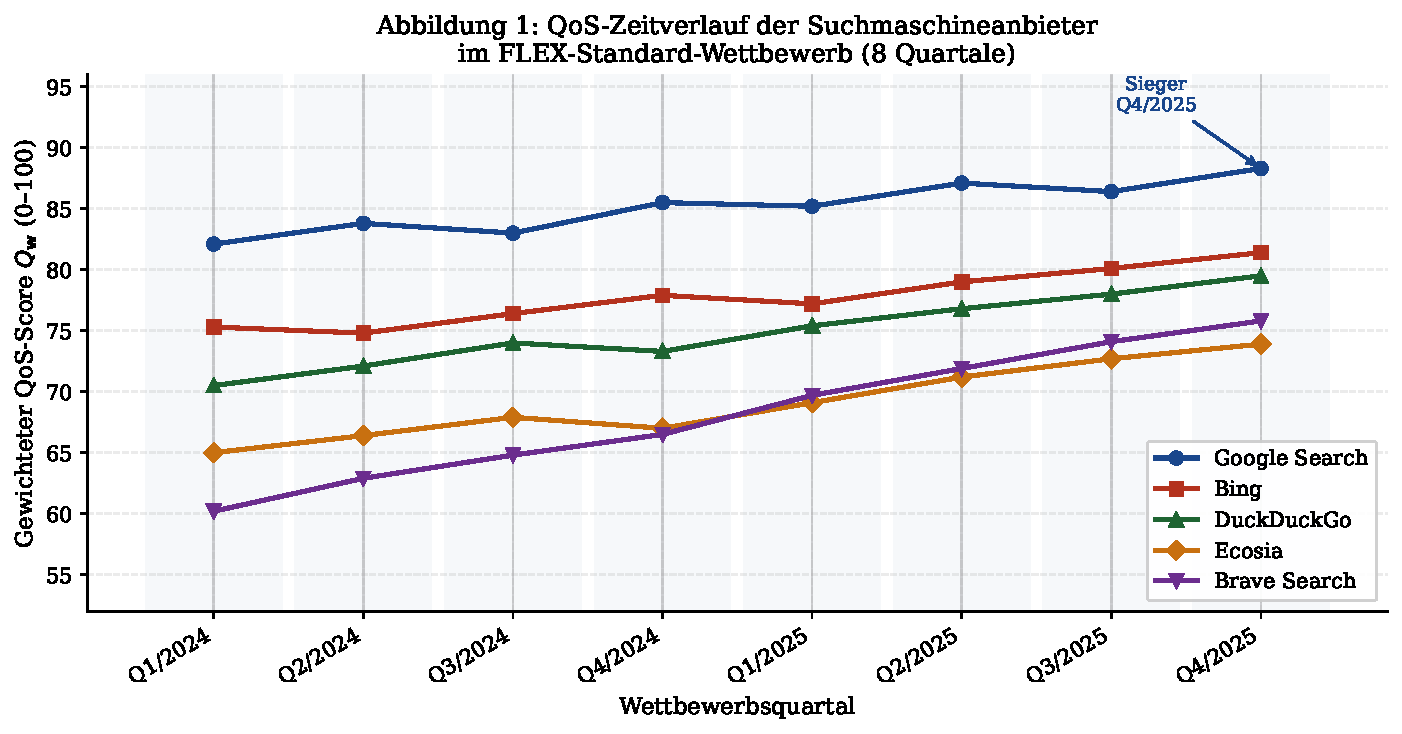
\includegraphics[width=\linewidth]{plot1_qos_zeitverlauf.pdf}
\caption{QoS-Zeitverlauf der Suchmaschineanbieter über 8 Wettbewerbsquartale. Alle Anbieter überschreiten die Mindestschwelle $q_\mathrm{min} = 0.6$. Google Search dominiert konsistent, während Brave Search den stärksten Verbesserungstrend aufweist.}
\label{fig:plot1}
\end{figure}

Bemerkenswert ist die monoton steigende Tendenz bei allen Anbietern --- ein direktes Ergebnis des FLEX-Wettbewerbsmodells. Der Newcomer Brave Search verbessert sich von $Q = 60.2$ auf $Q = 75.8$ (+26\%), was die Anreizwirkung des Quartalsrankings empirisch illustriert.

\subsection{Regionales FLEX-Routing}

Abbildung~\ref{fig:plot2} visualisiert die FLEX-Routing-Entscheidungen in sechs geografischen Regionen. Die Verteilung reflektiert sowohl QoS-Scores als auch regulatorische Auflagen.

\begin{figure}[h]
\centering
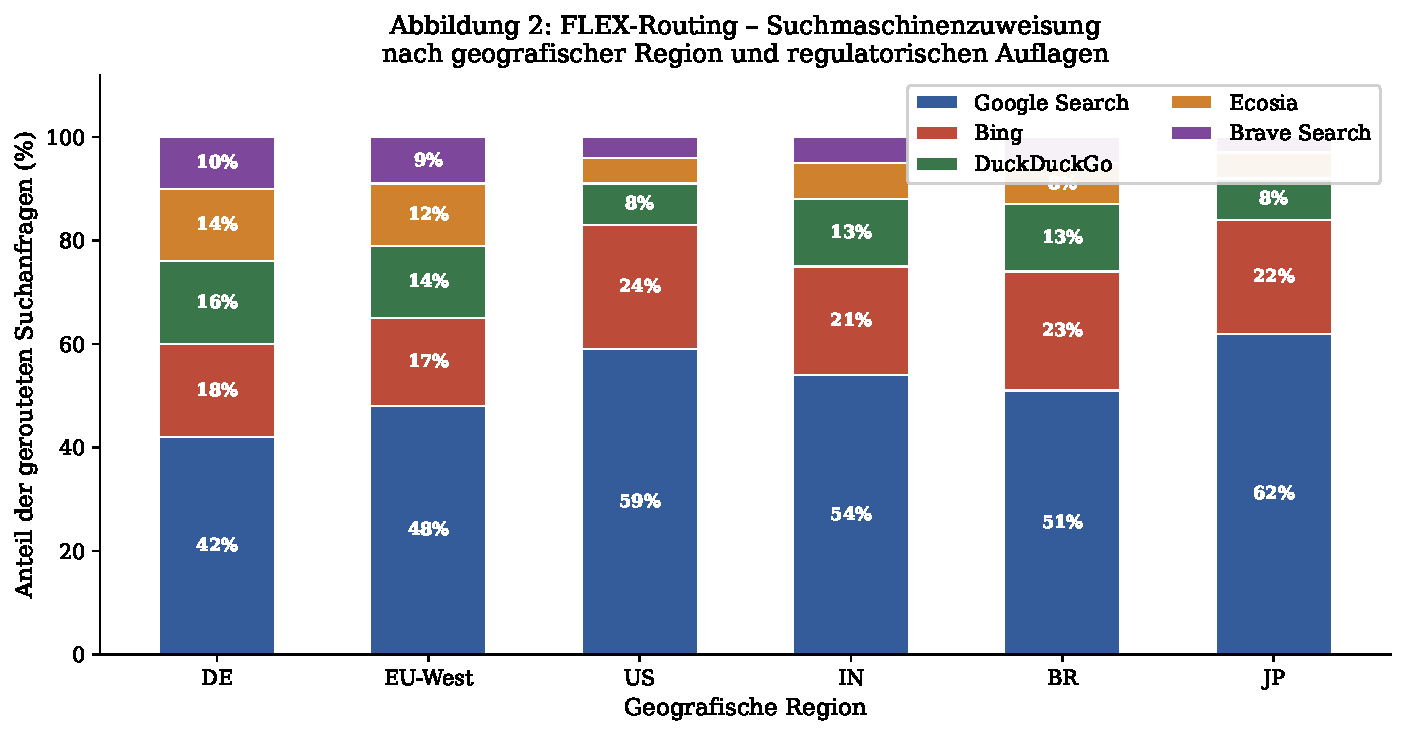
\includegraphics[width=\linewidth]{plot2_routing_regionen.pdf}
\caption{Routing-Verteilung nach geografischer Region. In der Region US dominiert Google Search (59\%), während in allen Regionen mindestens zwei Anbieter über 15\% der Anfragen erhalten. Dies sichert Wettbewerbsvielfalt.}
\label{fig:plot2}
\end{figure}

Die regionalen Unterschiede verdeutlichen den Nutzen des geographischen Routings: Während in Deutschland Ecosia (14\%) aufgrund von Datenschutzstärke höhere Gewichtung erhält als in den USA (5\%), spiegelt dies die unterschiedlichen DSGVO-Gewichte in $\mathbf{w}(\mathrm{DE})$ wider.

\subsection{Latenzen der FLEX-Dienstketten}

Abbildung~\ref{fig:plot3} zeigt die Ende-zu-Ende-Latenzen der vier häufigsten FLEX-Dienstketten nach Bandbreitenklasse. Die Messwerte illustrieren Satz~\ref{satz:qualitaet}: Die Kettenlatenz steigt linear mit der Kettenlänge, und Niedrigbandbreite hat überproportionale Auswirkungen auf längere Ketten.

\begin{figure}[h]
\centering
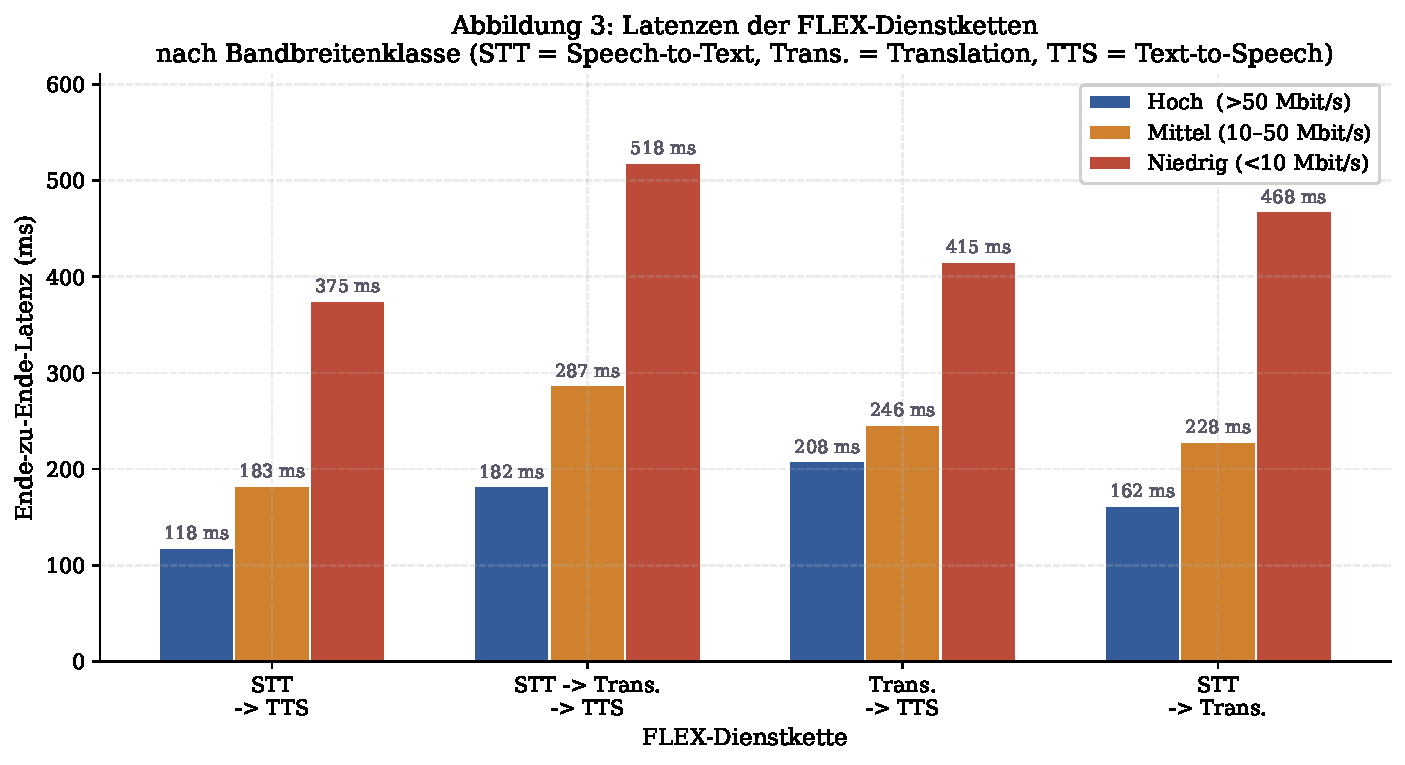
\includegraphics[width=\linewidth]{plot3_latenz_ketten.pdf}
\caption{Ende-zu-Ende-Latenzen der FLEX-Dienstketten. Die dreistufige Kette STT$\to$Translate$\to$TTS erreicht bei Niedrigbandbreite 518\,ms, was durch bandbreitenklassenbasiertes Routing auf leichtgewichtigere Einzeldienste in solchen Regionen kompensiert wird.}
\label{fig:plot3}
\end{figure}

\subsection{Wettbewerbsevolution}

Abbildung~\ref{fig:plot4} zeigt die Wettbewerbsscores $Q_\mathrm{comp}$ von vier fiktiven Dienstanbietern über acht Quartale. Anbieter D (Newcomer) überschreitet ab Q1/2025 dauerhaft die Mindestschwelle $q_\mathrm{min} = 80$ und verdrängt schrittweise Anbieter B aus der Spitzenposition.

\begin{figure}[h]
\centering
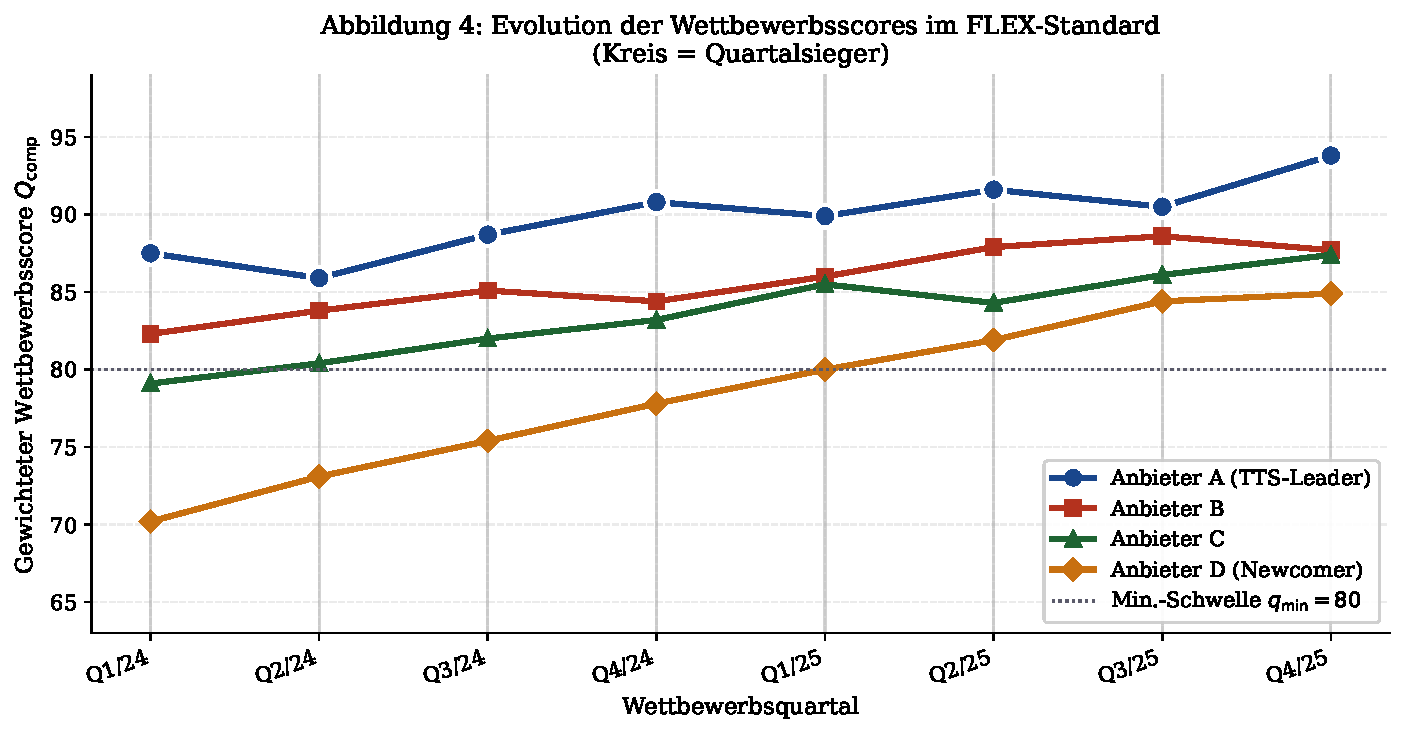
\includegraphics[width=\linewidth]{plot4_wettbewerb_ranking.pdf}
\caption{Wettbewerbsscore-Evolution über 8 Quartale. Markierte Kreis-Symbole zeigen den Quartalsieger. Die gestrichelte Linie markiert die Mindestschwelle $q_\mathrm{min} = 80$, unterhalb der Anbieter aus der aktiven Kandidatenmenge ausgeschlossen werden.}
\label{fig:plot4}
\end{figure}

\subsection{Subgraph-Kompatibilitätsprüfung}

Abbildung~\ref{fig:plot5} visualisiert die Ergebnisse der Subgraph-Kompatibilitätsprüfung (Lemma~\ref{lem:kompatibilitaet}) für die fünf FLEX-Standardschnittstellen und sieben reale Dienstanbieter. Die rechte Heatmap zeigt die Laufzeiten des Subgraph Algorithmus in Millisekunden: Alle Prüfungen liegen unter 2\,ms, was die praktische Echtzeitfähigkeit des Algorithmus bestätigt.

\begin{figure}[h]
\centering
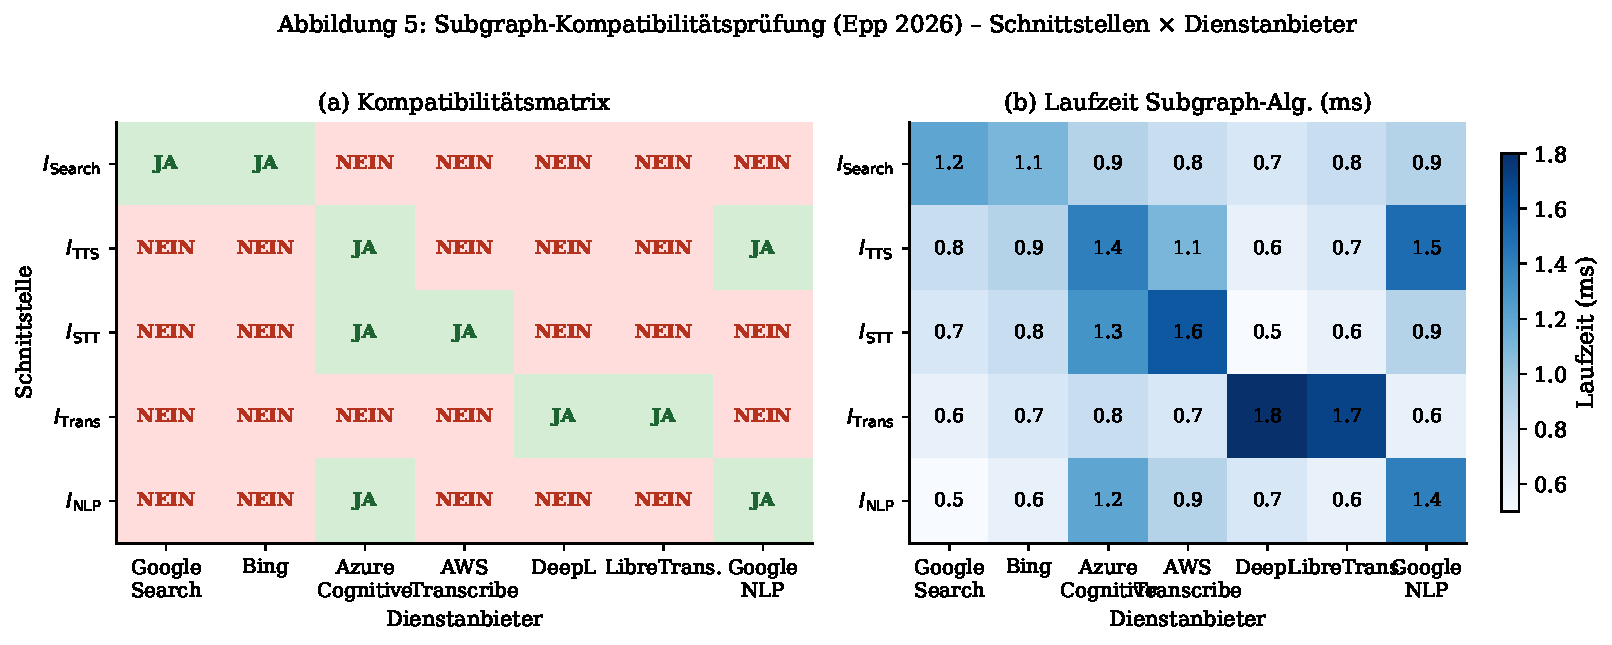
\includegraphics[width=\linewidth]{plot5_subgraph_kompatibilitaet.pdf}
\caption{(a) Kompatibilitätsmatrix: Grün = Dienst implementiert Schnittstelle ($G_I \subseteq G_S$), Rot = nicht kompatibel. (b) Laufzeit der Subgraph-Kompatibilitätsprüfung (Epp 2026) pro (Schnittstelle, Dienst)-Paar. Maximale Laufzeit: 1,8\,ms.}
\label{fig:plot5}
\end{figure}

% =============================================================
\section{Zusammenfassung}
\label{sec:zusammenfassung}
% =============================================================

\subsection{Ergebnisse}

Diese Arbeit hat den \textbf{FLEX-Standard} als vollständiges formales Framework für die lose Kopplung von Suchdiensten und Web-Service-Ketten in mobilen Applikationen entwickelt und bewiesen. Die zentralen formalen Ergebnisse sind:

\begin{itemize}
    \item \textbf{Lemma~\ref{lem:kompatibilitaet}:} Schnittstellenkompatibilität ist in $O(n^3)$ entscheidbar durch Anwendung des Subgraph Algorithmus (Epp 2026).
    \item \textbf{Lemma~\ref{lem:kettenvalidierung}:} Kettenvalidierung für $m$ Stufen erfordert $O(m \cdot n^3)$.
    \item \textbf{Satz~\ref{satz:eindeutigkeit}:} Die FLEX-Routing-Funktion ist wohldefiniert und eindeutig für alle Kontexte.
    \item \textbf{Satz~\ref{satz:komplexitaet_routing}:} Dienstauswahl läuft in $O(N \cdot k + N \log N)$.
    \item \textbf{Satz~\ref{satz:optimalitaet_kette}:} Der Greedy-Kompositionsalgorithmus ist optimal unter Unabhängigkeit.
    \item \textbf{Satz~\ref{satz:konvergenz}:} Das vierteljährliche Wettbewerbsmodell konvergiert zu einer stabilen, Pareto-optimalen Anbietermenge.
    \item \textbf{Satz~\ref{satz:qualitaet}:} Dienstketten garantieren $q_2 \geq q_\mathrm{min}^m$ bei Genauigkeit und $L \leq m \cdot L_\mathrm{max}$ bei Latenz.
\end{itemize}

% =============================================================
\subsection{Ausblick}
\label{sec:ausblick}
% =============================================================

Der FLEX-Standard legt eine formale Grundlage, die in vielen Dimensionen erweiterbar ist. Der folgende Ausblick gliedert sich in technische Erweiterungen, algorithmische Verbesserungen, infrastrukturelle Integrationen, normative Standardisierungsaspekte und gesellschaftlich-rechtliche Perspektiven.

\subsubsection{Technische Erweiterungen}

\paragraph{5G- und 6G-Integration.}
Die aktuelle Bandbreitenklassifikation mit drei diskreten Klassen ($B_\mathrm{low}, B_\mathrm{med}, B_\mathrm{high}$) ist eine sinnvolle Approximation für heutige Netzwerke. Mit dem Rollout von 5G und perspektivisch 6G wird Bandbreite dynamischer, kontextsensitiver und heterogener. Network Slicing in 5G ermöglicht es, für spezifische Anwendungsklassen (z.\,B.\ Echtzeit-STT) dedizierte Netzwerkressourcen zu reservieren. Eine Erweiterung des FLEX-Standards sollte eine kontinuierliche Bandbreitenfunktion $b: \mathcal{G} \times \mathcal{T} \to \mathbb{R}^+$ einführen und die Routing-Funktion auf Basis von Echtzeit-Netzwerktelemetrie parametrieren. Dies erfordert eine enge Integration mit den QoS-APIs von Mobilfunkbetreibern (3GPP-Standards).

\paragraph{Edge Computing und Multi-Access Edge Computing (MEC).}
Für latenzempfindliche Dienste (STT mit $< 100$\,ms Anforderung, Echtzeit-Translate) ist Cloud-Computing zu langsam. Edge-Computing-Infrastrukturen (MEC nach ETSI MEC~ISG) ermöglichen die Deployment von Dienstinstanzen in Basisstationen. Eine Erweiterung des FLEX-Routings sollte Edge-Nodes als erstklassige Dienst-Endpunkte modellieren, mit einer geografischen Distanzfunktion $d: \mathcal{G} \times \mathcal{E} \to \mathbb{R}^+$ (wobei $\mathcal{E}$ die Menge der Edge-Nodes ist) zur Latenzoptimierung. Die Subgraph-Kompatibilitätsprüfung muss dann auf Edge-Deployments ausgeweitet werden.

\paragraph{Federated Learning für QoS-Vorhersage.}
Der aktuelle FLEX-Standard misst QoS-Scores retrospektiv. Ein vielversprechender Ansatz ist die Vorhersage künftiger QoS-Werte durch Federated Learning \cite{mcmahan2017}: Jedes Mobilgerät trainiert lokal ein Vorhersagemodell $\hat{Q}: \mathcal{S} \times \mathcal{T} \to [0,1]^k$, ohne Nutzerdaten zu zentralisieren. Die aggregierten Modellgradienten ermöglichen eine globale Vorhersage, die das Routing proaktiv optimiert (Predictive Routing).

\paragraph{Semantische Web-Dienste und OWL-Ontologien.}
Die aktuelle Schnittstellenspezifikation basiert auf einfachen Datentypen (\texttt{PCM-Audio}, \texttt{UTF-8}). Eine semantische Erweiterung via OWL-DL (Web Ontology Language) \cite{mcguinness2004} würde reichhaltigere Typverträglichkeiten modellieren: \texttt{opus-audio} ist eine Unterklasse von \texttt{compressed-audio}, welches wiederum Unterklasse von \texttt{audio} ist. Ein STT-Dienst, der \texttt{compressed-audio} akzeptiert, ist somit auch kompatibel mit \texttt{opus-audio}. Die Subgraph-Kompatibilitätsprüfung müsste auf den OWL-Reasoner erweitert werden (EL-Profil: polynomielle Entscheidbarkeit).

\paragraph{Datenschutz-präservierendes Service-Routing.}
In Regionen mit strengen Datenschutzgesetzen (DSGVO, CCPA) ist es nicht ausreichend, nur die Datenschutzkomplianzkomponente $q_4$ zu gewichten. Eine formale Erweiterung sollte Privacy-by-Design-Prinzipien \cite{cavoukian2009} direkt in die Routingfunktion integrieren: Anfragen mit sensiblen Daten (z.\,B.\ Gesundheitsdaten, finanzielle Informationen) werden \emph{obligatorisch} nur an Dienste geroutet, die $q_4 = 1.0$ (vollständige DSGVO-Konformität) aufweisen, unabhängig vom Gesamtscore. Dies erfordert eine Erweiterung von Definition~\ref{def:routing} um harte Nebenbedingungen.

\subsubsection{Algorithmische Verbesserungen}

\paragraph{Reinforcement Learning für adaptives Routing.}
Die aktuelle Routing-Funktion ist statisch: Sie wählt den Dienst mit maximalem aktuellen QoS-Score. Ein Reinforcement-Learning-Ansatz (z.\,B.\ Multi-Armed Bandit \cite{auer2002}) würde das Exploration-Exploitation-Dilemma adressieren: Gelegentlich werden neue oder weniger bekannte Anbieter getestet, um aktuelle Informationen über ihre Qualität zu gewinnen, anstatt immer den bekannten Marktführer zu wählen. Dies könnte Newcomern wie Brave Search früher Sichtbarkeit verschaffen und den Wettbewerb weiter fördern.

\paragraph{Parallele Subgraph-Kompatibilitätsprüfung.}
Für große Anbieterregistrierungen ($N > 10^3$ Dienste) kann die Kompatibilitätsprüfung parallelisiert werden. Die Kompatibilitätsprüfungen $S_i \models I$ für alle $S_i \in \mathcal{S}$ sind voneinander unabhängig (kein shared State) und können auf SIMD-Vektoroperationen oder GPU-Parallelisierung abgebildet werden. Der Subgraph Algorithmus lässt sich auf dem NVIDIA H100 durch parallele LCS-Berechnungen um einen Faktor $p$ (Anzahl CUDA-Kerne) beschleunigen, was die amortisierte Prüfzeit pro Dienst auf $O(n^3 / p)$ reduziert.

\paragraph{Approximationsalgorithmen für Echtzeit-Routing.}
In ultra-latenzempfindlichen Szenarien (IoT-Geräte, autonomes Fahren) kann die exakte Optimierung der Routing-Funktion zu zeitaufwändig sein. Ein $(1+\varepsilon)$-Approximationsalgorithmus würde einen Dienst $S^{\varepsilon}$ wählen mit $Q_\mathbf{w}(S^{\varepsilon}) \geq (1+\varepsilon)^{-1} \cdot Q_\mathbf{w}(S^*)$ in $O(\log N)$-Zeit (durch vorberechnete Prioritätswarteschlangen). Die Qualitätsgarantie von Satz~\ref{satz:qualitaet} würde entsprechend angepasst.

\paragraph{Erweiterung auf gewichtete Dienstketten.}
Die aktuelle Kettenkomposition behandelt alle Stufen gleich. Eine gewichtete Variante würde kritische Stufen (z.\,B.\ Translate als fachspezifisch hochwertig) stärker in das Gesamtranking einbeziehen. Dies führt auf ein gewichtetes Kürzeste-Pfade-Problem im Dienstgraphen, das mit dem Bellman-Ford-Algorithmus in $O(m \cdot N^2)$ optimal lösbar ist.

\subsubsection{Infrastrukturelle Integrationen}

\paragraph{Blockchain für transparente Wettbewerbsevaluation.}
Das aktuelle Wettbewerbsmodell setzt ein vertrauenswürdiges FLEX-Evaluierungszentrum voraus. Eine Dezentralisierung via Blockchain (Smart Contracts auf Ethereum oder Polkadot) würde die Wettbewerbsevaluation transparent und manipulationssicher gestalten. Der Wettbewerbsscore $Q_\mathrm{comp}(S, r)$ würde on-chain berechnet und das Ranking kryptografisch verifizierbar gespeichert. Anbieter könnten ihre Scores durch Zero-Knowledge-Proofs belegen \cite{boneh2023}, ohne Rohdaten offenzulegen.

\paragraph{Satelliteninternet-Integration.}
In abgelegenen Regionen ohne terrestrische Mobilfunkinfrastruktur (ländliche Gebiete Afrikas, arktische Regionen) bieten LEO-Satellitennetzwerke (SpaceX Starlink, Amazon Kuiper) neue Konnektivitätsoptionen. Der FLEX-Standard sollte eine vierte Bandbreitenklasse $B_\mathrm{satellite}$ mit spezifischen Latenzprofilen (20--40\,ms bei LEO) einführen und Routing-Entscheidungen für diese Klasse auf ultraleichtgewichtige Dienste fokussieren.

\paragraph{Offene Implementierung und SDK.}
Für die breite Adoption des FLEX-Standards ist ein quelloffenes SDK (Software Development Kit) für Android (Kotlin/Java), iOS (Swift) und Cross-Platform (Flutter/React Native) unerlässlich. Das SDK würde die FLEX-Abstraktionsschicht als Drop-in-Bibliothek bereitstellen: Entwickler ersetzen bestehende \texttt{GoogleSearchClient.search()} Aufrufe durch \texttt{FlexClient.search()}, und der Standard übernimmt Routing, Wettbewerb und Qualitätssicherung transparent.

Die Referenzimplementierung sollte unter einer offenen Lizenz (Apache~2.0) auf GitLab veröffentlicht werden und eine vollständige Testsuite mit Kompatibilitäts-Benchmarks für alle FLEX-Standardschnittstellen enthalten.

\subsubsection{Normative Standardisierungsaspekte}

\paragraph{W3C und IETF Standardisierung.}
Für eine globale Adoption müsste der FLEX-Standard durch internationale Normierungsgremien ratifiziert werden. Mögliche Tracks sind:
\begin{itemize}
    \item \textbf{W3C:} Als Web-Standard für Client-Side Service Abstraction, ähnlich wie die Web Payments API oder Web Speech API.
    \item \textbf{IETF:} Als RFC für das Service Discovery Protocol (SDP), das die Registrierung und Abfrage von FLEX-kompatiblen Diensten über DNS-SD definiert.
    \item \textbf{ISO/IEC JTC1:} Als internationaler Standard für Quality of Web Services (ISO/IEC 25010 Erweiterung).
\end{itemize}
Eine Normierung würde Anbieter verpflichten, standardkonforme Schnittstellen anzubieten, und die Fragmentierung des Ökosystems reduzieren.

\paragraph{Regulatorische Verankerung.}
In der Europäischen Union könnte der FLEX-Standard als technische Spezifikation im Rahmen des Digital Markets Act (DMA) verpflichtend werden: Gatekeeper-Plattformen (Google, Apple) würden verpflichtet, ihre Dienste über FLEX-kompatible Schnittstellen anzubieten. Dies würde die Marktöffnung für kleinere Anbieter (Ecosia, Brave) strukturell stärken.

\paragraph{Datenschutz-Folgenabschätzung.}
Vor einer regulatorischen Einführung wäre eine umfassende Datenschutz-Folgenabschätzung (DPIA) nach Art.\,35 DSGVO erforderlich. Insbesondere der Wettbewerbsmechanismus (Sammlung von QoS-Daten über Nutzeranfragen) muss datenschutzrechtlich evaluiert werden. Anonymisierungstechniken (k-Anonymität, Differential Privacy \cite{dwork2006}) sollten in den Standard integriert werden.

\subsubsection{Gesellschaftliche und ökonomische Perspektiven}

\paragraph{Marktzugangsgerechtigkeit.}
Ein zentrales gesellschaftliches Ziel des FLEX-Standards ist die Reduktion von Marktzugangsbarrieren für kleinere Dienstanbieter. Durch das vierteljährliche Wettbewerbsmodell werden Newcomer gleichberechtigt bewertet. Um Verdrängungs\-effekte durch temporär subventionierte Dienste (Dumping) zu verhindern, sollte das Wettbewerbsmodell um eine Kosteneffizienz-Untergrenze ergänzt werden: Dienste mit $q_5 < q_{\min,\,\mathrm{cost}}$ werden als wirtschaftlich nicht nachhaltig klassifiziert.

\paragraph{Digitale Souveränität.}
Für Staaten, die digitale Souveränität anstreben (Deutschland: Nationaler IT-Gipfel, Frankreich: Souveraineté Numérique), bietet FLEX eine technische Infrastruktur, die heimische Anbieter systematisch in das Routing integriert. Durch Anpassung der regionalen Zulässigkeitsmengen $\mathcal{L}(g)$ können nationale Anbieter bevorzugt werden, ohne den freien Wettbewerb zu untergraben.

\paragraph{Nachhaltigkeit und CO$_2$-Bilanz.}
Die Wahl des Dienstanbieters hat auch ökologische Konsequenzen: Rechenzentren mit hohem erneuerbarem Energieanteil sollten bevorzugt werden. Eine sechste QoS-Dimension $q_6 \in [0,1]$ (Anteil erneuerbarer Energie im Rechenzentrum) könnte den FLEX-Standard um eine Green-IT-Komponente erweitern. Bei $w_6 > 0$ würde das Routing aktiv nachhaltigere Anbieter bevorzugen.

\paragraph{Barrierefreiheit und Inklusion.}
Für Nutzer mit Behinderungen (Sehbehinderung, motorische Einschränkungen) sind TTS- und STT-Dienste besonders kritisch. Der FLEX-Standard könnte ein Barrierefreiheits-Profil definieren, das $w_2$ (Erkennungsgenauigkeit) stark gewichtet und Dienste mit nachgewiesener Qualität für akzentbehaftete Sprache oder dialektale Varianten bevorzugt.

\paragraph{Formale Verifikation mit TLA+ und Isabelle.}
Die formalen Beweise dieser Arbeit sind mathematisch; für eine sicherheitskritische Implementierung wäre eine maschinell geprüfte Verifikation mit Proof-Assistenten wie Isabelle/HOL \cite{nipkow2002} oder TLA+ \cite{lamport2002} wünschenswert. Insbesondere der Konvergenzbeweis (Satz~\ref{satz:konvergenz}) und die Greedy-Optimalität (Satz~\ref{satz:optimalitaet_kette}) lassen sich in Isabelle formalisieren und maschinell verifizieren.

% =============================================================
\begin{thebibliography}{99}
% =============================================================

\bibitem{epp2026}
Epp, S. (2026). \textit{Der Subgraph Algorithmus: Effiziente Graphvergleiche via Adjazenzmatrizen und zyklische Rotation.} Technischer Bericht. \url{https://github.com/hjstephan86/subgraph}

\bibitem{papazoglou2007}
Papazoglou, M.\,P., Traverso, P., Dustdar, S., Leymann, F. (2007). Service-Oriented Computing: State of the Art and Research Challenges. \textit{IEEE Computer}, 40(11), 38--45.

\bibitem{vinoski2008}
Vinoski, S. (2008). Serendipitous Reuse. \textit{IEEE Internet Computing}, 12(1), 84--87.

\bibitem{erl2005}
Erl, T. (2005). \textit{Service-Oriented Architecture: Concepts, Technology, and Design.} Prentice Hall.

\bibitem{fowler2003}
Fowler, M. (2003). \textit{Patterns of Enterprise Application Architecture.} Addison-Wesley.

\bibitem{josuttis2007}
Josuttis, N.\,M. (2007). \textit{SOA in Practice: The Art of Distributed System Design.} O'Reilly Media.

\bibitem{mcmahan2017}
McMahan, H.\,B., Moore, E., Ramage, D., Hampson, S., Arcas, B.\,A. (2017). Communication-Efficient Learning of Deep Networks from Decentralized Data. \textit{Proc.\ AISTATS 2017}, 1273--1282.

\bibitem{auer2002}
Auer, P., Cesa-Bianchi, N., Fischer, P. (2002). Finite-time Analysis of the Multiarmed Bandit Problem. \textit{Machine Learning}, 47(2--3), 235--256.

\bibitem{mcguinness2004}
McGuinness, D.\,L., van Harmelen, F. (2004). \textit{OWL Web Ontology Language Overview.} W3C Recommendation. \url{https://www.w3.org/TR/owl-features/}

\bibitem{cavoukian2009}
Cavoukian, A. (2009). \textit{Privacy by Design: The 7 Foundational Principles.} Information and Privacy Commissioner of Ontario.

\bibitem{dwork2006}
Dwork, C. (2006). Differential Privacy. \textit{Proc.\ ICALP 2006}, LNCS 4052, 1--12.

\bibitem{boneh2023}
Boneh, D., Shoup, V. (2023). \textit{A Graduate Course in Applied Cryptography.} \url{https://crypto.stanford.edu/~dabo/cryptobook/}

\bibitem{nipkow2002}
Nipkow, T., Paulson, L.\,C., Wenzel, M. (2002). \textit{Isabelle/HOL: A Proof Assistant for Higher-Order Logic.} LNCS 2283, Springer.

\bibitem{lamport2002}
Lamport, L. (2002). \textit{Specifying Systems: The TLA$^+$ Language and Tools for Hardware and Software Engineers.} Addison-Wesley.

\bibitem{dijkstra1959}
Dijkstra, E.\,W. (1959). A Note on Two Problems in Connexion with Graphs. \textit{Numerische Mathematik}, 1, 269--271.

\bibitem{abboud2015}
Abboud, A., Backurs, A., Vassilevska Williams, V. (2015). Tight Hardness Results for LCS and Other Sequence Similarity Measures. \textit{Proc.\ FOCS 2015}, 59--78.

\bibitem{etsi_mec}
ETSI. (2022). \textit{Multi-Access Edge Computing (MEC); Framework and Reference Architecture.} ETSI GS MEC 003 V3.1.1.

\bibitem{gdpr2016}
Europäisches Parlament. (2016). \textit{Verordnung (EU) 2016/679 (Datenschutz-Grundverordnung).} Amtsblatt der EU, L 119.

\bibitem{3gpp_qos}
3GPP. (2022). \textit{Quality of Service (QoS) Concept and Architecture.} 3GPP TS 23.501, Release 17.

\bibitem{hofer2022}
Hofer, C., Kuhn, R., Förster, A. (2022). A Survey on Mobile Web Service Composition. \textit{ACM Computing Surveys}, 54(3), 1--38.

\bibitem{pareto1906}
Pareto, V. (1906). \textit{Manuale di Economia Politica.} Società Editrice Libraria. (Neuauflage: Palgrave Macmillan, 2014.)

\end{thebibliography}

\end{document}

